% Created 2014-09-27 Sat 01:02
\documentclass[11pt]{article}
\usepackage[utf8]{inputenc}
\usepackage[T1]{fontenc}
\usepackage{fixltx2e}
\usepackage{graphicx}
\usepackage{longtable}
\usepackage{float}
\usepackage{wrapfig}
\usepackage{rotating}
\usepackage[normalem]{ulem}
\usepackage{amsmath}
\usepackage{textcomp}
\usepackage{marvosym}
\usepackage{wasysym}
\usepackage{amssymb}
\usepackage{hyperref}
\tolerance=1000
\usepackage[utf8]{inputenc}
\usepackage[a4paper]{geometry}
\usepackage[usenames,dvipsnames]{color}
\usepackage[11pt]{moresize}
\usepackage{minted}
\usemintedstyle{perldoc}
\hypersetup{urlcolor=blue}
\hypersetup{colorlinks,urlcolor=blue}
\setlength{\parskip}{16pt plus 2pt minus 2pt}
\definecolor{codebg}{rgb}{0.96,0.99,0.8}
\author{Oleg Sivokon}
\date{2014-08-24}
\title{Science Versus Magic}
\hypersetup{
  pdfkeywords={PowToon Model Improvement Prolog},
  pdfsubject={Creating better models with automated tools},
  pdfcreator={Emacs 24.3.50.1 (Org mode 8.2.2)}}
\begin{document}

\maketitle
\tableofcontents


\newpage

\section{The conflict}
\label{sec-1}

\begin{figure}[h!]
  \centering
  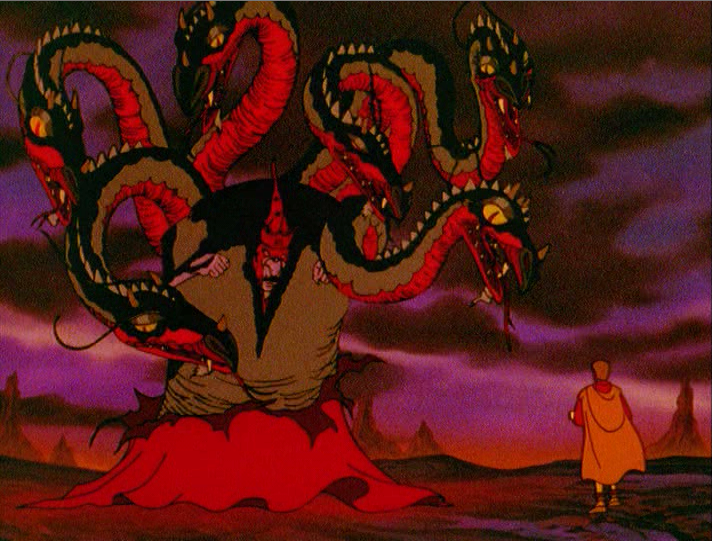
\includegraphics[width=0.8\textwidth]{./the-flight-of-dragons.png}
  \caption[Magic vs Science]{
    \ssmall Maigc (on the left) versus science (on the right).
    \textit{The final battle from The Flight of Dragons,
      a 1982 animated film produced by Jules Bass and Arthur Rankin, Jr.}}
\end{figure}

The dawn of 19'th century was the tipping point in the battle of logicians
versus magicians.  While logicians won, the battle isn't of the kind that wins
the war.  The war still rages on in each of the human minds.  But do we have
to bow before our new overlords?  What are the consequences of doing so?
Or should we, perhaps, die fighting?

\subsection{The history of the conflict}
\label{sec-1-1}

\begin{figure}[h!]
  \centering
  
\includegraphics[width=0.8\textwidth]{./insect-overlords.png}
  \caption[Welcome insect overlords]{
    \ssmall ``And I for one welcome our new insect overlords''
    \textit{A statement made by Kent Brockman, a Channel 6 news anchor in
      the 1994 episode of The Simpsons, ``Deep Space Homer''}}
\end{figure}

Even though the system of formal proof was known as early as Ancient Greece,
due to the work of Euclid---who laid foundations of geometry and the modern
day formal reasoning, it was not until Frege that formal reasoning become a
requirement, first for logic and mathematics and later, with the help from
philosophers such as Rudolf Carnap and Karl Popper, it become a requirement
for natural sciences.  These ideas were furthered by Jan Paul Sartr, who
built upon Friedrich Nietzsche's earlier works, which suggested that
phenomenalism must be abandoned.  The idea, which had a profound effect on
human sciences.  Combined with Piagetian approach to teaching and development
of an individual it demystified the process of thinking.  This, in turn,
enabled Alan Turing to conceive of a \emph{universal} theory of computation, that
is to extend thinking beyond humanity, to level it with other natural events
such as those which would be described by physcis or biology.

Of course, the magic didn't surrender its positions willingly! Occasionally
its guerilla warfare gained enough strenght to overthrow the new regime.
Although so far, most such cases had been contained, eventually the hydra
would raise its head like the phoenix from ashes, stare at you blankly with
the eyes the size of teacups and then plunge back into the depths of despair
from whence it came, carrying you along on its feathered beak.

\noindent\rule{\textwidth}{0.5pt}

The pennant of science flies proudly into the face of the scattered and
receding foes.  Its champions herald victory.  Alan Kay, leading the charge
with his Croquet project, and \url{http://www.opencobalt.org/} to follow.  The
arrays of \url{http://code.org} marching onward chanting

\begin{verse}
  \itshape
  Mess with the best (tum, tum) \\
  Die like the rest (tum, tum) \\
  Rah, rah, rah!
\end{verse}
\subsection{The tempation}
\label{sec-1-2}

\begin{figure}[h!]
  \centering
  
\includegraphics[width=0.8\textwidth]{./Might-and-Magic-Heroes-VI-Angel.jpg}
  \caption[HOMM VI promo poster]{
    \ssmall A promo poster for the game Heroes of Might and Magic VI.}
\end{figure}

I admit that magic is cool.

\begin{figure}[h!]
  \centering
  
\includegraphics[width=0.8\textwidth]{./mlp.jpg}
  \caption[MLP season 2 episode 8]{
    \ssmall The promo poster released for My Little Pony: 
    Friendship is Magic series.
    \textit{Second season, Episode 8.}}
\end{figure}

And some times even cooler.

Magic is the best possible solution to any kind of problem we might come up
with.  Even by the standards of science, there is no plausible reason not to
choose magic, since it offers an easier solution.  Doing things the
scientific way is remarkably harder.  But what makes magic so easy and
appealing?

\begin{itemize}
\item We've inherited most of it.  The will to believe in magic runs in our
veings.  It is the heirloom of our ancestors that we cherish and love so
fondly that makes it a moral imperative to believe in magic.
\item There seems to be a natural tendency in the way of how humans approach
problem solving to prefer some algorithms over others.  In particular,
humans strongly discriminate against all algorithms which suggest more than
added logarithmic time.  We also favor myopic decisions, which seems to be
due to the benefits of finding any being greater than the costs associated
with search that will likely take a very long time.
\item The very fact that anyone of us survived thus far ignites a belief
that by doing what we did until this point we are guaranteed a greater
chance of success than by following any other strategy.
\item On top of that, there's the peer pressure.  As long as we are convinced that 
our peers will accept our magical thinking as a valid approach to
describing reality, we are safe in our beliefs.  We don't require complete
agreement to validate our belief system.  A smiple acknowledgment of the
method's validity is enough for magic to proliferate.
\item Finally, magic is ubiquotous, it is forgiving, it is pervasive.  
Quantitatively, it occupies infinitely larger fraction of the solution
space than the one left to the science.  So, even if you don't choose
sides, by the virtue of sheer chance alone, you would most likely end up
doing magic.
\end{itemize}

Science, on the other hand, nags you, repremands you whenever you fall short
of attaining its standards which seem to never stop getting higher.  It pays
no repsect to traditions or religions.  It can't be bothered with the mood
swings of your boss or the fact that you have a family to feed.  It offers
hard work and ever so rarely an elusive reward.  It isn't something you can
easily pass on to your heirs, in fact, it becomes more difficult with each
generation to even preserve that what has been found.  It is
counterintuitive, it is rare and fragile.  So why would you even consider
choosing it?

\emph{(Nevermind, it was a rhetorical question)}. The \emph{reason} you should choose\ldots{}
oh wait, do you notice what's going on here: we are talking about, I'll
emphasize it again, the \emph{REASON}.  Isn't it obvious that to to talk about
what the \emph{reason} is, we should know what the reason \emph{is}?  And that would
be by doing scinece!  But there's another way to answer the question:
magic is bad, and here's why.

\newpage
\subsection{Why magic is bad}
\label{sec-1-3}

\begin{figure}[h!]
  \centering
  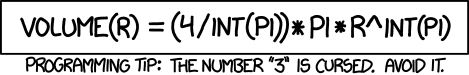
\includegraphics[width=0.8\textwidth]{./int_pi.png}
  \caption[Cursed number 3]{
    \ssmall \url{http://xkcd.com/1275/}}
\end{figure}

You probably watched at least one movie urging you to believe in magic.  Even
the expression ``believe in magic'' itself is too catchy to have possibly
escaped your attention.  It is a far less known fact that the word ``magic''
has a negative or pejorative meaning, when used by programmers.  In that
later sense, ``magic'' means something that cannot be explained rationally.
``Magic numbers'' are numbers that appear in a program for no discernible
reason.  The same goes for strings.  The reasons for dislike are simple:
magic does not allow one to solve the problem mechanically.  Mechancial
solutions are based on the fact that the problem can be formulated logically,
that is \emph{formalized!} If there is a number in one's program without an
explanation of how to produce it, that number is magical.  What is meant by
that is: that whoever will try to adapt the program to their need will have
to answer the question \emph{should this number be the same for me, or should I
draw a different one?} Given the infinite nature of numbers, the question may
not be answered through guessing (magic).
\subsection{Inventor paradox}
\label{sec-1-4}

\begin{figure}[h!]
  \centering
  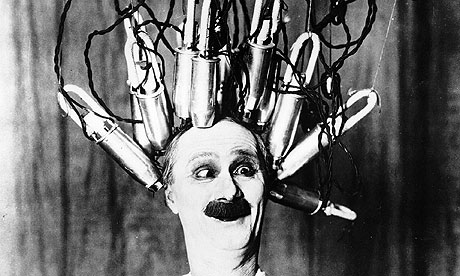
\includegraphics[width=0.8\textwidth]{./electorshocked-inventor.jpg}
  \caption[Inventor-chopper]{
    \ssmall Bernard Turpin as a mad scientist}
\end{figure}

In a nutshell, inventor paradox is the observation that, despite what you
might expect, once the subject of one's research is more constrained it
becomes easier to proceed to finding solution.  A way of understanding why
this happens is to think that the unconstrained parts of the problem are
\emph{magical} in the same sense, in which numbers or strings can be (as discussed
in \ref{sec-1-3}.)  Once the search space becomes infinitely large, it
becomes impossible to make any progress.  We've invented formalization as a
response to the problem posed by infinity.  In fact, despite all the
hardship, there is no better way to cope with infinity.  No matter what Soren
Kierkegaard have you believe.
\subsection{Magical thinking}
\label{sec-1-5}

\begin{figure}[h!]
  \centering
  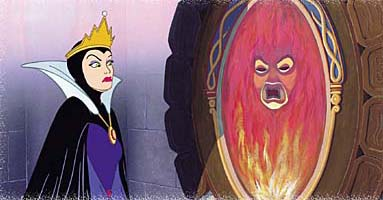
\includegraphics[width=0.8\textwidth]{./queen.jpg}
  \caption[Mirror, mirror on the wall...]{
    \ssmall The evil queen consulting the magic mirror.
    \textit{A scene from Walt Disney 1937 film 
      Snow White and the Seven Dwarfs}}
\end{figure}

Magical thinking is the extension of magical numbers and strings.  Magical
thinking is understood as reliance on superstition, religious belief or
exercise of some religious rite, witnessing a revelation, being in a transe,
or by observing a taboo.  But some times it's not easy to recognize it as
such.  Quasi-religious practices are not in themselves a source of magical
thinking, they are a fertile ground for one.  It flourishes due to all the
same reasons descirbed in \ref{sec-1-2}.

Unfortunately, we already know, that to follow this route is to sink in the
abyss of infinite choices, the despair of uncertain, meaningless existence.

Nevertheless, there is hope.  Generations after generations, despite eventual
defeats, periods of stagnation and highly unreliable infrastructre, it seems
like the determination of the few had preserved and even improved the
scientific knowledge.  The next chapter of this pamphlet is an attempt to
pass some of it onward.

\newpage
\section{The solution}
\label{sec-2}

In order to convince you of the practical benefits of formalization over magic
I hereby present you the model of the PowToon player UI.  I've spent about an
hour constructing it, verifying its correctness and putting down related
notes.

First, lets commit to the memory these vocabulary words:

\begin{itemize}
\item \emph{symbol} or \emph{term} is the basic unit of the Prolog program.  By convention
symbols start with a lowercase letter, but you can go against the
convention, if you so want, in which case you will have to wrap them in
single quotes.
\item Prolog can define a \emph{fact}.  A fact is either a symbol, a relation (note that
symbols are nullary relations too), or a recurrence (a complex kind of
relation).  The later two are also refered to as \emph{rules} or \emph{clauses}.
\item All facts of a \emph{program} constitute a \emph{database}.
\item Therefore, your program can add facts to the database, or \emph{query} the database
to derive new facts.  Queries start with \texttt{?-} symbol.
\end{itemize}

\subsection{Database}
\label{sec-2-1}

Now, define some facts about what we know to be true for the player:

\begin{minted}[bgcolor=codebg,fontsize=\scriptsize]{prolog}
playback(playing).
playback(stopped).
\end{minted}

\emph{The player can either play or pause}.

\begin{minted}[bgcolor=codebg,fontsize=\scriptsize]{prolog}
position(beginning).
position(middle).
position(end).
\end{minted}

\emph{The playhead can be positioned at the beginning of the timeline, at the end}
\emph{or somewhere in the middle}.

\begin{minted}[bgcolor=codebg,fontsize=\scriptsize]{prolog}
content(slide).
content(video).
\end{minted}

\emph{At any given moment the contents of the player are either video, or anything}
\emph{else, which I choose to describe as slide}.

\begin{minted}[bgcolor=codebg,fontsize=\scriptsize]{prolog}
mode(auto).
mode(manual).
\end{minted}

\emph{Finally, the player can be either in auto-play or manual modes}.

Now, lets sum it all up:

\begin{minted}[bgcolor=codebg,fontsize=\scriptsize]{prolog}
modifiers(Playback, Position, Content, Mode):-
    playback(Playback),
    position(Position),
    content(Content),
    mode(Mode).
\end{minted}

\emph{The state of the player is a combination of its playback, its position, its}
\emph{content and its mode}.
\subsection{Constraints}
\label{sec-2-2}

Now, lets put some constraints in place.  This is the interesting part.  Here we
define what things we don't want to happen in the player.  Specifically, we are
interested in that certain buttons will not be visible in certain states.

\begin{minted}[bgcolor=codebg,fontsize=\scriptsize]{prolog}
first_button(modifiers(_, Position, _, _), Button):-
    ( Position = beginning -> Button = none ; Button = rewind ).

second_button(modifiers(Playback, Position, Content, _), Button):-
    ( Position = end -> Button = replay ;
      ( Playback = stopped ->
        ( Content = video -> Button = play_video ; Button = play_slide ) ;
        ( Content = video -> Button = stop_video ; Button = stop_slide ) ) ).

third_button(modifiers(_, Position, _, _), Button):-
    ( Position = end -> Button = none ; Button = fast_forward ).

fourth_button(modifiers(_, _, _, Mode), Button):-
    ( Mode = auto -> Button = auto ; Button = manual ).
\end{minted}

Whoa, this was a lot of code for one time, let's see what it does!

\emph{This code assumes there are four slots for buttons we are interested in.}
\emph{First slot can be either empty or occupied by} \texttt{rewind} \emph{button.  Second}
\emph{slot can be occupied by a whole five different buttons.  Third slot is}
\emph{very similar to the first one, and the last one is never empty, but switches}
\emph{between} \texttt{auto} \emph{and} \texttt{manual} \emph{buttons}.

Note the constructions \texttt{( condition -> goal1 ; goal2 )}. Also note new
vocabulary word \emph{goal}.  Goals are \emph{propositions} that we \emph{prove} by executing
the program.  Effectively, our program is a mechanical tool for proving formal
statements made about the \emph{universe of discourse} (or a \emph{structure}) defined
in the program.  The sentence above could be thus read as follows:

\emph{If it is possible to prove} \texttt{condition} \emph{then prove} \texttt{goal1}, \emph{otherwise}
\emph{prove} \texttt{goal2}.
\subsection{Larger example}
\label{sec-2-3}

\begin{minted}[bgcolor=codebg,fontsize=\scriptsize]{prolog}
if_pressed(Button, modifiers(Playback, Position, Content, Mode), NextState):-
    ( Button = none ->
      NextState = modifiers(Playback, Position, Content, Mode) ;
      Button = rewind ->
      ( Position = middle ->
        NextState = modifiers(Playback, beginning, Content, Mode) ;
        NextState = modifiers(Playback, middle, Content, Mode) ) ;
      Button = fast_forward ->
      ( Position = middle ->
        NextState = modifiers(Playback, end, Content, Mode) ;
        NextState = modifiers(Playback, middle, Content, Mode) ) ;
      Button = play_video ->
      ( Content = video ,
        Playback = stopped ,
        ( Position = middle ; Position = beginning ) ,
        NextState = modifiers(playing, Position, Content, Mode) ) ;
      Button = stop_video ->
      ( Content = video , Playback = playing ,
        ( Position = middle ; Position = beginning ) ,
        NextState = modifiers(stopped, Position, Content, Mode) ) ;
      Button = play_slide ->
      ( Content = slide , Playback = stopped ,
        ( Position = middle ; Position = beginning ) ,
        NextState = modifiers(playing, Position, Content, Mode) ) ;
      Button = stop_slide ->
      ( Content = slide , Playback = playing ,
        ( Position = middle ; Position = beginning ) ,
        NextState = modifiers(playing, Position, Content, Mode) ) ;
      Button = replay ->
      ( Position = end ,
        NextState = modifiers(stopped, beginning, Content, Mode) ) ;
      Button = auto ->
      ( Mode = auto ,
        NextState = modifiers(Playback, Position, Content, manual) ) ;
      Button = manual ->
      ( Mode = manual ,
        NextState = modifiers(Playback, Position, Content, auto) ) ).
\end{minted}

   Even though we've defined the behavior of the buttons, we are still nowhere
near making our program useful.  Below is a first attempt at putting it all
together:

Whoa, this was a lot of code! But, to tell you the truth, this code could
have been condenced to a fraction of the above by use of recursion.
Recursion is universally acknowledged to be a hard topic for beginners, and
this is one of the reasons why the code is presented as a list of rules
rather than a more condence and mathematically appealing form.  If you
examine it closely you will see that the code is largerly repetitive, thus
doesn't require as much effort understanding it as was the case with the
previous snippets.

All this rule does it encodes the behavior of buttons, when they are pressed in
various states.  Now, this is what we were after!  Finally, this is a really
useful program.  This program can unambiguously answer questions such as:

\emph{What should the UI look like, given its previous state and the fact}
\emph{that the} \texttt{fast\_forward} \emph{button was clicked?}

Compare this to the existing document.  Which one is longer? Which one can be
reliably said to capture all possible cases?  Which one can be used mechanically
to develop a program and to verify that the program meets the requirements?
Know that it is only the beginning.  It is possible to do much, much more than
this, if only you apply some effort!
\subsection{Queries}
\label{sec-2-4}

Below are some examples of the queries one can execute against the database
defined above:

\begin{minted}[bgcolor=codebg,fontsize=\scriptsize]{prolog}
?- if_pressed(fast_forward, modifiers(stopped, middle, slide, manual), X).
X = modifiers(stopped, end, slide, manual).
\end{minted}

Reading:

\emph{What must be the state of the player UI, given that the previous state was}
\emph{such that the player didn't play, the playhead was in the middle of the}
\emph{timeline, the currently displayed content was a slide and the playback mode}
\emph{was manual}.

The answer given seems to be self-explanatory.

Even more, you can refine the question by asking specifically about the
change in position:

\begin{minted}[bgcolor=codebg,fontsize=\scriptsize]{prolog}
?- if_pressed(fast_forward,
              modifiers(stopped, middle, slide, manual),
              modifiers(_, X, _, _)).
X = end.
\end{minted}

Or, you could omit some detail of specification, to obtain more possible
answers:

\begin{minted}[bgcolor=codebg,fontsize=\scriptsize]{prolog}
?- if_pressed(play_video,
              modifiers(stopped, From, video, auto),
              modifiers(playing, To, video, auto)).
From = To, To = middle ;
From = To, To = beginning.
\end{minted}

The interpretation of the above:

\emph{The effect of pressing} \texttt{play\_video} \emph{button, given it is at all possible}
\emph{is such that if the player was in the} \texttt{middle} \emph{state, it will remain in}
\emph{the same state, and the same is true for} \texttt{beginning} \emph{state}.

From above you can also indirectly derive that this operation is not defined
for the \texttt{end} state, since this state doesn't allow us to press \texttt{play\_video}
button.
\subsection{Homework}
\label{sec-2-5}

But we aren't done yet!  The program can be augmented with the notion of
player's state, which also includes the state of the buttons:

\begin{minted}[bgcolor=codebg,fontsize=\scriptsize]{prolog}
buttons(State, [A, B, C, D]):-
    first_button(State, A),
    second_button(State, B),
    third_button(State, C),
    fourth_button(State, D).

state(Modifiers, Buttons):-
    modifiers(Modifiers), buttons(Modifiers, Buttons).
\end{minted}

Given this as a start, and usign the example from \ref{sec-2-3}, you can come
up with a program, which can answer questions like:

\emph{Given the player is in a particular state, and such-and-such buttons are visible}
\emph{what are the possible actions that can be taken to transition to the next state?}

Which I leave as an exercise for the reader.
% Emacs 24.3.50.1 (Org mode 8.2.2)
\end{document}
